\documentclass[a4paper,12pt]{article}
\special{papersize=210mm,297mm}

\usepackage[a4paper,top=1.45cm,bottom=1.7cm,left=1.85cm,right=1.85cm]{geometry}
\usepackage[fleqn]{amsmath}
\usepackage{amssymb}
\usepackage{array}
\usepackage{tabularx}
\usepackage{enumitem}
\usepackage{multicol}
\usepackage{needspace}
\usepackage{fontspec}
\usepackage{graphicx}
\usepackage{tikz}
\usetikzlibrary{arrows.meta}

\setmainfont{Times New Roman}
\setsansfont{Arial}
\setlength{\parindent}{0pt}
\setlength{\parskip}{0.12em}
\setlength{\mathindent}{0pt}
\linespread{1.04}
\emergencystretch=2em
\pagestyle{plain}

\newlength{\problemnumberwidth}
\settowidth{\problemnumberwidth}{\textbf{10.}\ }
\newcommand{\problem}[2]{%
  \Needspace{4\baselineskip}%
  \par\vspace{1.05em}%
  \noindent
  \hangindent=\problemnumberwidth\relax
  \hangafter=1
  \makebox[\problemnumberwidth][l]{\textbf{#1.}}#2\par
}
\newcommand{\answerline}{\rule{4cm}{0.4pt}}
\newcommand{\tableheadcell}[1]{\rule[-0.35em]{0pt}{1.55em}\textbf{#1}}
\newcommand{\functioncell}[1]{\rule[-1.35em]{0pt}{3.1em}\(\displaystyle #1\)}
\newcolumntype{Y}{>{\centering\arraybackslash}X}
\newcolumntype{C}[1]{>{\centering\arraybackslash}m{#1}}

\newcommand{\maclaurintable}{%
  \par\vspace{0.75em}%
  \noindent\hspace*{\problemnumberwidth}%
  \begin{minipage}{\dimexpr\textwidth-\problemnumberwidth\relax}
  \setlength{\tabcolsep}{5pt}%
  \setlength{\arrayrulewidth}{0.45pt}%
  \renewcommand{\arraystretch}{1.05}%
  \begin{tabularx}{\linewidth}{|C{0.22\linewidth}|Y|C{0.20\linewidth}|}
    \hline
    \tableheadcell{Function} &
    \tableheadcell{Maclaurin Series} &
    \tableheadcell{Radius of conv.} \\
    \hline
    \functioncell{e^x} & & \\
    \hline
    \functioncell{\cos{} x} & & \\
    \hline
    \functioncell{\dfrac{1}{1+x}} & & \\
    \hline
    \functioncell{\arctan{} x} & & \\
    \hline
    \functioncell{\ln(1+x)} & & \\
    \hline
    \functioncell{\sin{} x} & & \\
    \hline
    \functioncell{{(1+x)}^k} & & \\
    \hline
  \end{tabularx}
  \end{minipage}\par
}

\newlist{subparts}{enumerate}{1}
\setlist[subparts]{%
  label={(\alph*)},
  leftmargin=2.4em,
  labelsep=0.6em,
  itemsep=0.55em,
  topsep=0.55em,
  parsep=0pt
}
\newlist{romanparts}{enumerate}{1}
\setlist[romanparts]{%
  label={(\roman*)},
  leftmargin=2.4em,
  labelsep=0.6em,
  itemsep=0.65em,
  topsep=0.65em,
  parsep=0pt
}
\newlist{choices}{enumerate}{1}
\setlist[choices]{%
  label={(\Alph*)},
  leftmargin=2.6em,
  labelsep=0.6em,
  itemsep=0.28em,
  topsep=0.42em,
  parsep=0pt
}
\newcommand{\serieschoices}{%
  \par\vspace{0.25em}%
  \noindent
  \begin{tabularx}{\linewidth}{@{}>{\raggedright\arraybackslash}X>{\raggedright\arraybackslash}X>{\raggedright\arraybackslash}X@{}}
    (A) absolutely convergent &
    (B) conditionally convergent &
    (C) divergent
  \end{tabularx}%
  \par\vspace{0.2em}%
}

\newcommand{\contourmapfigure}{%
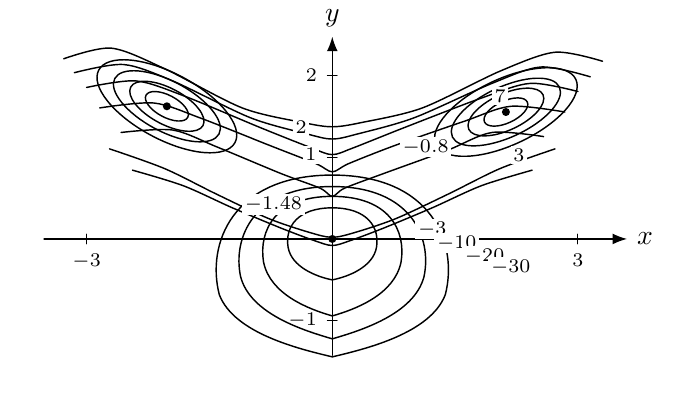
\begin{tikzpicture}[x=1.04cm,y=1.04cm,>=Latex,line cap=round,line join=round]
  \tikzset{contour/.style={line width=0.52pt}}

  \path[use as bounding box] (-3.72,-1.55) rectangle (3.82,2.58);

  \draw[->,line width=0.5pt] (-3.52,0) -- (3.60,0) node[right] {\(x\)};
  \draw[->,line width=0.5pt] (0,-1.42) -- (0,2.47) node[above] {\(y\)};
  \foreach \x/\lab in {-3/-3,3/3} {
    \draw[line width=0.35pt] (\x,0.06) -- (\x,-0.06);
    \node[below] at (\x,-0.06) {\scriptsize \(\lab\)};
  }
  \foreach \y/\lab in {-1/-1,1/1,2/2} {
    \draw[line width=0.35pt] (0.06,\y) -- (-0.06,\y);
    \node[left] at (-0.07,\y) {\scriptsize \(\lab\)};
  }

  \draw[contour] plot[smooth] coordinates {(-3.28,2.20) (-2.70,2.33) (-2.05,2.08) (-1.10,1.60) (-0.35,1.42) (0,1.37) (0.35,1.42) (1.10,1.60) (2.05,2.05) (2.72,2.28) (3.30,2.17)};
  \draw[contour] plot[smooth] coordinates {(-3.15,2.03) (-2.55,2.13) (-1.95,1.93) (-1.00,1.48) (-0.30,1.28) (0,1.22) (0.30,1.28) (1.00,1.48) (1.95,1.90) (2.55,2.10) (3.15,1.98)};
  \draw[contour] plot[smooth] coordinates {(-3.00,1.85) (-2.40,1.93) (-1.82,1.75) (-0.88,1.36) (-0.25,1.11) (0,1.03) (0.25,1.11) (0.88,1.36) (1.82,1.72) (2.42,1.90) (3.00,1.80)};
  \draw[contour] plot[smooth] coordinates {(-2.84,1.60) (-2.18,1.66) (-1.62,1.48) (-0.76,1.14) (-0.20,0.92) (0,0.82) (0.20,0.92) (0.76,1.14) (1.62,1.44) (2.18,1.62) (2.84,1.55)};
  \draw[contour] plot[smooth] coordinates {(-2.58,1.30) (-1.95,1.33) (-1.40,1.12) (-0.63,0.80) (-0.15,0.62) (0,0.52) (0.15,0.62) (0.63,0.80) (1.40,1.08) (1.95,1.30) (2.58,1.25)};

  \draw[contour] plot[smooth] coordinates {(-2.72,1.10) (-2.05,0.86) (-1.42,0.55) (-0.78,0.25) (-0.28,0.08) (0,0.02) (0.28,0.08) (0.78,0.25) (1.42,0.55) (2.05,0.86) (2.72,1.10)};
  \draw[contour] plot[smooth] coordinates {(-2.44,0.84) (-1.82,0.65) (-1.22,0.38) (-0.62,0.13) (-0.22,-0.02) (0,-0.08) (0.22,-0.02) (0.62,0.13) (1.22,0.38) (1.82,0.65) (2.44,0.84)};

  \foreach \rx/\ry in {0.30/0.14,0.52/0.23,0.75/0.32,0.98/0.42} {
    \draw[contour,rotate around={-28:(-2.02,1.62)}]
      (-2.02,1.62) ellipse[x radius=\rx cm,y radius=\ry cm];
  }
  \foreach \rx/\ry in {0.30/0.14,0.52/0.23,0.75/0.32,0.98/0.42} {
    \draw[contour,rotate around={25:(2.12,1.55)}]
      (2.12,1.55) ellipse[x radius=\rx cm,y radius=\ry cm];
  }

  \draw[contour]
    (0,0.38)
    .. controls (-0.42,0.38) and (-0.58,0.15) .. (-0.54,-0.10)
    .. controls (-0.50,-0.34) and (-0.20,-0.46) .. (0,-0.50)
    .. controls (0.20,-0.46) and (0.50,-0.34) .. (0.54,-0.10)
    .. controls (0.58,0.15) and (0.42,0.38) .. (0,0.38);
  \draw[contour]
    (0,0.52)
    .. controls (-0.70,0.52) and (-0.90,0.10) .. (-0.84,-0.28)
    .. controls (-0.76,-0.68) and (-0.28,-0.86) .. (0,-0.94)
    .. controls (0.28,-0.86) and (0.76,-0.68) .. (0.84,-0.28)
    .. controls (0.90,0.10) and (0.70,0.52) .. (0,0.52);
  \draw[contour]
    (0,0.64)
    .. controls (-0.96,0.64) and (-1.22,0.02) .. (-1.12,-0.46)
    .. controls (-1.00,-0.92) and (-0.34,-1.12) .. (0,-1.22)
    .. controls (0.34,-1.12) and (1.00,-0.92) .. (1.12,-0.46)
    .. controls (1.22,0.02) and (0.96,0.64) .. (0,0.64);
  \draw[contour]
    (0,0.78)
    .. controls (-1.22,0.78) and (-1.54,-0.06) .. (-1.38,-0.68)
    .. controls (-1.20,-1.15) and (-0.42,-1.34) .. (0,-1.44)
    .. controls (0.42,-1.34) and (1.20,-1.15) .. (1.38,-0.68)
    .. controls (1.54,-0.06) and (1.22,0.78) .. (0,0.78);

  \fill (-2.02,1.62) circle[radius=1.45pt];
  \fill (2.12,1.55) circle[radius=1.45pt];
  \fill (0,0) circle[radius=1.45pt];

  \node[fill=white,inner sep=1pt] at (2.05,1.74) {\scriptsize \(7\)};
  \node[fill=white,inner sep=1pt] at (2.28,1.02) {\scriptsize \(3\)};
  \node[fill=white,inner sep=1pt] at (-0.38,1.37) {\scriptsize \(2\)};
  \node[fill=white,inner sep=1pt] at (-0.26,1.03) {\scriptsize \(1\)};
  \node[fill=white,inner sep=1pt] at (1.14,1.12) {\scriptsize \(-0.8\)};
  \node[fill=white,inner sep=1pt] at (-0.72,0.42) {\scriptsize \(-1.48\)};
  \node[fill=white,inner sep=1pt] at (1.22,0.12) {\scriptsize \(-3\)};
  \node[fill=white,inner sep=1pt] at (1.52,-0.05) {\scriptsize \(-10\)};
  \node[fill=white,inner sep=1pt] at (1.86,-0.21) {\scriptsize \(-20\)};
  \node[fill=white,inner sep=1pt] at (2.18,-0.35) {\scriptsize \(-30\)};
\end{tikzpicture}%
}

\newcommand{\polarregionfigure}{%
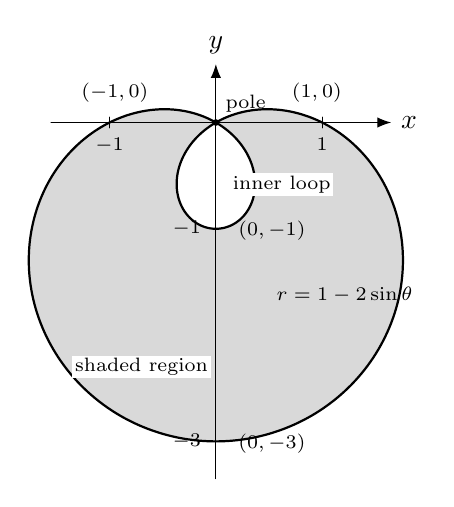
\begin{tikzpicture}[x=1.35cm,y=1.35cm,>=Latex,line cap=round,line join=round]
  \fill[gray!30]
    plot[domain=150:390,samples=260,variable=\t]
      ({(1 - 2*sin(\t))*cos(\t)}, {(1 - 2*sin(\t))*sin(\t)})
    -- cycle;
  \fill[white]
    plot[domain=30:150,samples=160,variable=\t]
      ({(1 - 2*sin(\t))*cos(\t)}, {(1 - 2*sin(\t))*sin(\t)})
    -- cycle;

  \draw[->,line width=0.45pt] (-1.55,0) -- (1.65,0) node[right] {\(x\)};
  \draw[->,line width=0.45pt] (0,-3.35) -- (0,0.55) node[above] {\(y\)};
  \draw[line width=0.35pt] (-1,0.05) -- (-1,-0.05) node[below] {\scriptsize \(-1\)};
  \draw[line width=0.35pt] (1,0.05) -- (1,-0.05) node[below] {\scriptsize \(1\)};
  \draw[line width=0.35pt] (0.05,-1) -- (-0.05,-1) node[left] {\scriptsize \(-1\)};
  \draw[line width=0.35pt] (0.05,-3) -- (-0.05,-3) node[left] {\scriptsize \(-3\)};

  \draw[black,thick]
    plot[domain=150:390,samples=260,variable=\t]
      ({(1 - 2*sin(\t))*cos(\t)}, {(1 - 2*sin(\t))*sin(\t)});
  \draw[black,thick]
    plot[domain=30:150,samples=160,variable=\t]
      ({(1 - 2*sin(\t))*cos(\t)}, {(1 - 2*sin(\t))*sin(\t)});

  \fill (0,0) circle[radius=1.2pt] node[above right] {\scriptsize pole};
  \node[right] at (0.48,-1.62) {\scriptsize \(r=1-2\sin\theta\)};
  \node[fill=white,inner sep=1pt] at (0.62,-0.58) {\scriptsize inner loop};
  \node[fill=white,inner sep=1pt] at (-0.70,-2.30) {\scriptsize shaded region};
  \node[right] at (0.12,-3.02) {\scriptsize \((0,-3)\)};
  \node[right] at (0.12,-1.02) {\scriptsize \((0,-1)\)};
  \node[above] at (0.95,0.10) {\scriptsize \((1,0)\)};
  \node[above] at (-0.95,0.10) {\scriptsize \((-1,0)\)};
\end{tikzpicture}%
}

\begin{document}

\begin{center}
  {\Large\bfseries Winter Term Calculus Midterm}\\
  {\large\bfseries (Science and Engineering)}\\[0.35em]
  April 23, 2026\\[1.55em]
  Show all your work except for Problems 1-5.
\end{center}

\problem{1}{Write down the Maclaurin series of the following functions and indicate the radius of convergence.}

\maclaurintable{}

\problem{2}{Circle all the vectors which are normal to the vector \(\langle 1,2,3\rangle\) in \(\mathbb{R}^3\).}

\[
\langle 3,0,-1\rangle \qquad
\langle 1,-2,1\rangle \qquad
\langle 0,-3,2\rangle \qquad
\langle 4,-2,0\rangle \qquad
\langle 1,-1,1\rangle
\]

\Needspace{20\baselineskip}
\problem{3}{Multiple choice problems.}

\begin{romanparts}
  \item \begin{minipage}[t]{\linewidth}
  Suppose the contour map of \(f(x,y)\) is given in Figure 1. How many saddle points of \(f(x,y)\) are presented here?

  \begin{multicols}{6}
  \begin{choices}
    \item \(0\)
    \item \(1\)
    \item \(2\)
    \item \(3\)
    \item \(4\)
    \item \(5\)
  \end{choices}
  \end{multicols}

  \begin{center}
    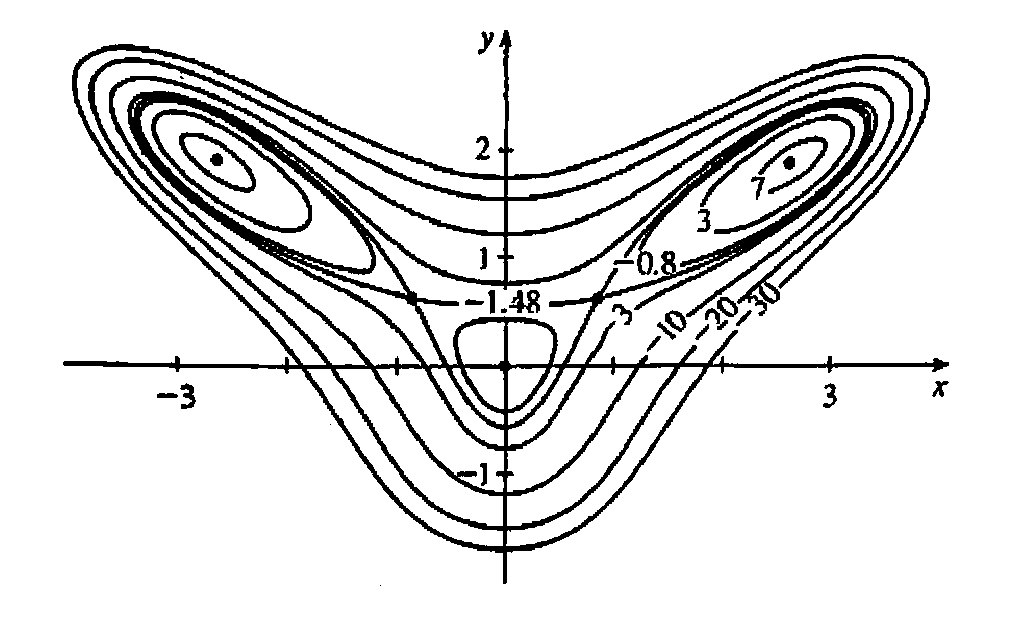
\includegraphics[width=7.6cm]{3i.png}

    \smallskip
    {\small\bfseries Figure 1.} {\small The contour map of \(f(x,y)\)}
  \end{center}
  \end{minipage}

  \item The series \(\displaystyle \sum_{n=0}^{\infty}{(-1)}^n\dfrac{n}{\sqrt{3n^2+n-3}}\) is

  \serieschoices{}

  \item The series \(\displaystyle \sum_{n=2}^{\infty}\dfrac{{(-1)}^n}{n{(\ln n)}^2}\) is

  \serieschoices{}

  \item The series \(\displaystyle \sum_{n=1}^{\infty}\dfrac{\cos(n\pi)}{n}\) is

  \serieschoices{}

  \item The series \(\displaystyle \sum_{n=1}^{\infty}{(-1)}^n\dfrac{100^n}{n!}\) is

  \serieschoices{}

  \Needspace{10\baselineskip}
  \item[(xiii)] \(\displaystyle \binom{1/2}{4}=\text{?}\)

  \begin{multicols}{4}
  \begin{choices}
    \item \(\dfrac{5}{2^4}\)
    \item \(-\dfrac{5}{2^4}\)
    \item \(\dfrac{5}{2^5}\)
    \item \(-\dfrac{5}{2^5}\)
    \item \(\dfrac{5}{2^6}\)
    \item \(-\dfrac{5}{2^6}\)
    \item \(\dfrac{5}{2^7}\)
    \item \(-\dfrac{5}{2^7}\)
  \end{choices}
  \end{multicols}
\end{romanparts}

\Needspace{17\baselineskip}
\problem{4}{Let \(f(x)=\dfrac{1}{{(1-2x^2)}^5}\). Suppose \(f^{(10)}(0)=a\binom{-5}{k}2^n\).}

\begin{romanparts}
  \item \(a=\) \answerline{}
  \item \(k=\) \answerline{}
  \item \(n=\) \answerline{}
\end{romanparts}

\begin{multicols}{4}
\begin{choices}
  \item \(1\)
  \item \(-1\)
  \item \(5\)
  \item \(-5\)
  \item \(10\)
  \item \(-10\)
  \item \(20\)
  \item \(-20\)
  \item \(5!\)
  \item \(-5!\)
  \item \(10!\)
  \item \(-10!\)
  \item \(\dfrac{1}{10!}\)
  \item \(-\dfrac{1}{10!}\)
  \item \(\dfrac{1}{5!}\)
  \item \(-\dfrac{1}{5!}\)
\end{choices}
\end{multicols}

\problem{5}{Find an error bound for the approximation \(\displaystyle \sin x\approx x-\dfrac{x^3}{3!}+\dfrac{x^5}{5!}\) when \(-0.2<x<0.2\).}

\problem{6}{}

\begin{subparts}
  \item Find the Maclaurin series of \(f(x)=x\sin x\) and give its interval of convergence.

  \item Integrate the series in (a) to show that
  \[
    \sum_{n=0}^{\infty}\dfrac{{(-1)}^n\pi^{2n+2}}{{(2n+1)}!(2n+3)}=1.
  \]
\end{subparts}

\problem{7}{Suppose given the cycloid}

\[
x=\theta-\sin\theta,\qquad y=1-\cos\theta,\qquad \theta\in\mathbb{R}.
\]

\begin{subparts}
  \item Find \(\dfrac{dy}{dx}\).
  \item Find \(\dfrac{d^2y}{dx^2}\) and simplify.
  \item Set up the definite integral for the arc length of one arch of the cycloid. Please simplify the integrand as much as possible.
\end{subparts}

\problem{8}{Let}

\[
f(x,y)=
\begin{cases}
\dfrac{xy}{x^2+y^2}, & \text{if }(x,y)\ne(0,0),\\[0.8em]
0, & \text{if }(x,y)=(0,0).
\end{cases}
\]

\begin{subparts}
  \item Find \(\displaystyle\lim_{(x,y)\to(0,0)} f(x,y)\).
  \item Is \(f(x,y)\) continuous at \((0,0)\)?
\end{subparts}

\problem{9}{The cardioid \(r=1-2\sin\theta\) is shown below:}

\begin{center}
  \polarregionfigure{}
\end{center}

\begin{subparts}
  \item Find \(\dfrac{dy}{dx}\).
  \item Set up the definite integral for the area of the shaded region.
\end{subparts}

\end{document}
